% !TEX program = xelatex

% \documentclass{cumcmthesis}
\documentclass[withoutpreface,bwprint]{cumcmthesis} %去掉封面与编号页,电子版提交的时候使用。


\usepackage[framemethod=TikZ]{mdframed}
\usepackage{url}   % 网页链接
\usepackage{subcaption} % 子标题
\title{全国大学生数学建模竞赛编写的 \LaTeX{} 模板}
% \tihao{A}
% \baominghao{4321}
% \schoolname{XX大学}
% \membera{ }
% \memberb{ }
% \memberc{ }
% \supervisor{ }%辅导老师
% \yearinput{2023}
% \monthinput{9}
% \dayinput{8}

\begin{document}

\maketitle
\begin{abstract}
    本题目针对碳化硅外延层厚度的无损伤测量,使用红外干涉法。问题1要求建立基于单次反射的厚度确定数学模型;问题2基于该模型设计算法,计算附件1和2中碳化硅晶圆片的厚度,并分析可靠性;问题3推导多光束干涉的必要条件及其对计算精度的影响,分析附件3和4中硅晶圆片是否出现多光束干涉,给出相应模型和计算结果;若认为多光束干涉也影响碳化硅数据,则需消除其影响并重新计算厚度。数据来自附件,提供波数和反射率。
    \keywords{\TeX{}\quad  图片\quad   表格\quad  公式}
\end{abstract}

%\newpage

\section{模板的基本使用}

要使用 \LaTeX{} 来完成建模论文,首先要确保正确安装一个 \LaTeX{} 的发行版本。

\begin{itemize}
    \item Mac 下可以使用 Mac\TeX{}
    \item Linux 下可以使用 \TeX{}Live ;
    \item windows 下可以使用 \TeX{}Live 或者 Mik\TeX{} ;
\end{itemize}

具体安装可以参考 \href{https://github.com/OsbertWang/install-latex-guide-zh-cn/releases/}{Install-LaTeX-Guide-zh-cn} 或者其它靠谱的文章。另外可以安装一个易用的编辑器,例如 \href{https://mirrors.tuna.tsinghua.edu.cn/github-release/texstudio-org/texstudio/LatestRelease/}{\TeX{}studio} 。

使用该模板前,请阅读模板的使用说明文档。下面给出模板使用的大概样式。

\begin{tcode}
    \documentclass{cumcmthesis}
    %\documentclass[withoutpreface,bwprint]{cumcmthesis} %去掉封面与编号页

    \title{论文题目}
    \tihao{A}            % 题号
    \baominghao{4321}    % 报名号
    \schoolname{你的大学}
    \membera{成员A}
    \memberb{成员B}
    \memberc{成员C}
    \supervisor{指导老师}
    \yearinput{2017}     % 年
    \monthinput{08}      % 月
    \dayinput{22}        % 日

    \begin{document}
    \maketitle
    \begin{abstract}
        摘要的具体内容。
        \keywords{关键词1\quad  关键词2\quad   关键词3}
    \end{abstract}
    \tableofcontents
    \section{问题重述}
    \subsection{问题的提出}
    \section{模型的假设}
    \section{符号说明}
    \begin{center}
        \begin{tabular}{cc}
            \hline
            \makebox[0.3\textwidth][c]{符号} & \makebox[0.4\textwidth][c]{意义} \\ \hline
            D                              & 木条宽度(cm)                       \\ \hline
        \end{tabular}
    \end{center}
    \section{问题分析}
    \section{总结}
    \begin{thebibliography}{9}%宽度9
        \bibitem{bib:one} ....
    \end{thebibliography}
    \begin{appendices}
        附录的内容。
    \end{appendices}
    \end{document}
\end{tcode}

根据要求,电子版论文提交时需去掉封面和编号页。可以加上 \verb|withoutpreface|  选项来实现,即:
\begin{tcode}
    \documentclass[withoutpreface]{cumcmthesis}
\end{tcode}
这样就能实现了。打印的时候有超链接的地方不需要彩色,可以加上 \verb|bwprint| 选项。

另外目录也是不需要的,将 \verb|\tableofcontents| 注释或删除,目录就不会出现了。

团队的信息填入指定的位置,并且确保信息的正确性,以免因此白忙一场。

编译记得使用 \verb|xelatex|,而不是用 \verb|pdflatex|。在命令行编译的可以按如下方式编译:
\begin{tcode}
    xelatex example
\end{tcode}
或者使用 \verb|latexmk| 来编译,更推荐这种方式。
\begin{tcode}
    latexmk -xelatex example
\end{tcode}

下面给出写作与排版上的一些建议。

%\newpage
\section{问题重述}
碳化硅(SiC)作为第三代半导体的核心材料,其外延层的厚度是决定器件性能的关键参数之一。精确、无损地测量外延层厚度在半导体工业中具有重要意义。红外干涉法因其高精度和非破坏性而被广泛应用。该方法的基本原理是:当红外光入射到SiC外延层时,光束会在外延层的上、下两个界面(空气-外延层界面与外延层-衬底界面)发生反射和折射,形成多束反射光。这些反射光之间因光程差而产生干涉,使得最终探测到的总反射光强度随光的波长(或波数)呈现周期性振荡,形成干涉光谱。本题旨在基于给定的干涉光谱数据,建立数学物理模型,反演出薄膜材料的厚度。具体任务如下:
\begin{enumerate}
    \item \textbf{基础模型构建与求解}:首先,在仅考虑上、下界面单次反射的理想情况下,建立干涉光谱与外延层厚度、材料折射率、入射角及光波数之间的数学模型。并利用该模型,对附件1和2中给出的碳化硅晶圆片在不同入射角下的干涉光谱数据进行分析,求解其外延层厚度。
    \item \textbf{精确模型构建与分析}:考虑到光束在薄膜内部可能发生多次反射的物理现实,建立一个更为精确的多光束干涉模型。基于新模型,从理论上分析其求解外延层厚度的可行性与算法设计。
    \item \textbf{模型泛化与应用}:探究多光束干涉效应变得显著的物理条件。进而,将所建立的多光束干涉模型应用于附件3和4中给出的硅(Si)晶圆片的光谱数据,计算其厚度,以验证模型的普适性。
    \item \textbf{数据处理与模型修正}:识别并量化碳化硅光谱数据中存在的多光束干涉等“次要效应”。设计并实施一种有效的信号处理算法,从原始光谱数据中滤除这些干扰,提取出主要由单次干涉决定的光谱信息。最后,基于净化后的数据,重新利用基础模型计算碳化硅外延层的精确厚度。
\end{enumerate}


\section{模型假设}

为了简化物理现实并建立可求解的数学模型,我们基于题目描述和光学原理,做出以下合理假设。每条假设附以理由和潜在风险,以确保模型的逻辑自洽性和鲁棒性。这些假设主要服务于问题一的单次反射模型,并在后续问题中逐步放松或扩展。

\begin{itemize}
    \item \textbf{几何结构理想化假设:}
          \begin{enumerate}
              \item \textbf{厚度均匀性:} 假设外延层在其被测量的区域内具有均匀一致的厚度 $d$。
              \item \textbf{界面平行且光滑:} 假设外延层的上表面(与空气接触)和下表面(与衬底接触)均为理想的光学平面,且彼此严格平行。这保证了反射和折射遵循几何光学定律。
          \end{enumerate}
    \item \textbf{材料光学特性假设:}
          \begin{enumerate}
              \item \textbf{光学均匀性与各向同性:} 假设外延层和衬底材料在光学上是均匀且各向同性的,即其折射率等光学参数在空间上不发生变化。
              \item \textbf{无吸收假设:} 假设在所研究的红外光谱范围内,外延层材料对光的吸收可以忽略不计。这意味着光在介质中传播时,其强度不会因材料吸收而衰减。
          \end{enumerate}
    \item \textbf{针对问题一的简化假设:}
          \begin{enumerate}
              \item \textbf{单次干涉模型:} 严格遵循题目要求,在构建基础模型时,仅考虑在空气-外延层界面反射的光束(反射光1)与在外延层-衬底界面反射一次后透出的光束(反射光2)之间的干涉,忽略所有后续的多次反射效应。
              \item \textbf{折射率恒定:} 假设外延层的折射率 $n$ 在所研究的波数范围内是一个常数,不随波数(波长)的变化而改变。这是一个关键的简化,旨在建立一个初步的、可解析的模型。
          \end{enumerate}

   
\end{itemize}
这些假设共同构成了我们分析问题的基础。其中,针对问题一的简化假设(如折射率恒定和单次干涉)将在后续问题的探讨中被逐步修正或放宽,以建立更符合物理实际的精确模型。

\section{符号说明}

\begin{center}
    \begin{tabular}{clll}
        \toprule
        符号        & 含义     & 单位          & 说明                            \\
        \midrule
        $d$       & 外延层厚度  & $\mu$m 或 nm & 待求解的核心变量                      \\
        $\nu$     & 波数     & cm$^{-1}$   & 数据第一列,等于 $1/\lambda$ (波长的倒数)  \\
        $R$       & 反射率    & \%          & 数据第二列,干涉光谱的测量值                \\
        $n$       & 外延层折射率 & —           & 随波长和掺杂浓度变化                    \\
        $\theta$  & 入射角    & $^\circ$    & 如 10$^\circ$ 或 15$^\circ$     \\
        $\lambda$ & 波长     & $\mu$m      & 与波数相关:$\lambda = 1/\nu$(注意单位) \\
        $\delta$  & 光程差    & m           & $\delta = 2 n d \cos \phi$    \\
        $m$       & 干涉级次   & —           & 整数                            \\
        \bottomrule
    \end{tabular}
\end{center}


\section{模型的建立与求解}

\subsection{问题一:平行平面薄膜双光束干涉的外延层厚度模型}

\subsubsection{光的振动函数}
时间变化的规律可以通过正弦函数和余弦函数来表述,其数学表达式为:

\[\overrightarrow{x}(t) = Acos(\omega t + \varphi)\]

\(\overrightarrow{x}(t)\):表示振动质点相对于其平衡位置的偏移量,用于描述质点在时刻 t 的位置。

\(A\) :光矢量的大小表示振动质点偏离其平衡位置的最大距离,以米为单位,反映了振动的强度。

\(\omega\) :角频率用于表征振动的速率,其单位为弧度/秒。它与频率 \(\nu\) 周期 \(T\) 的关系为 \(\omega = 2\pi\nu = \frac{2\pi}{T}\)。

\(\varphi\) :初相位是指在t=0时刻的相位,单位为弧度,用于确定振动的初始条件。

\subsubsection{光的振动描述——旋转矢量法}
如图1所示,采用旋转矢量法表示,一矢量绕原点O以角速度$\omega$逆时针匀速旋转,其瞬时在x轴上的投影即为光振动的简谐运动方程。

\begin{figure}[ht]
    \centering
    \fbox{\rule{2cm}{0pt} \rule{0pt}{2cm}} % 占位符用于图像
    \caption{旋转矢量法表示光的振动方程}
    \label{fig:1}
\end{figure}

如图1所示,该图通过旋转矢量法(亦称相量法)阐述了简谐振动的两种等效表示。左侧为几何表示:一振幅为$A$的矢量绕原点O以角频率$\omega$逆时针匀速旋转,其瞬时相位为$\phi=\omega t$。该矢量在纵轴(x轴)上的投影,即代表了振动系统在该时刻的瞬时位移x右侧为对应的时域表示,描述了上述投影随时间$t$的变化关系。如图所示,旋转矢量的运动精确地映射为一条以时间$t$为横轴、位移$x$为纵轴的正弦(或余弦)曲线,其数学表达为$x(t)=A\cos(\omega t+\varphi)$,与投影计算的结果完全一致。

旋转矢量法作为连接匀速圆周运动与一维简谐振动的桥梁,为理解振动参量提供了直观的几何图像:振幅$A$映射为旋转半径,决定了振动的强度;角频率 $\omega$映射为旋转角速度,决定了振动的快慢;初相位$\phi_0$映射为初始角位置,决定了振动的初始状态。这些几何关系清晰地解释了其时域波形$x(t)=A\cos(\omega t+\phi_0)$的特征。

\subsubsection{同方向同频率的光的合成}
考虑两个在同一直线上、具有相同角频率 $\omega$ 的简谐振动,其振动方程分别为:
$ \overrightarrow{x_1}(t) = A_1 \cos(\omega t + \phi_{1})$,其中 $A_1$ 是第一个振动的振幅, $\omega$ 是角频率, $\phi_{1}$ 是初相位;
$\overrightarrow{x_2}(t) = A_2 \cos(\omega t + \phi_{2})$,其中 $A_2$ 是第二个振动的振幅, $\phi_{2}$ 是初相位。合位移 $\overrightarrow{x}(t)$ 是两个分位移的矢量和,即 $\overrightarrow{x}(t) = \overrightarrow{x_1}(t) + \overrightarrow{x_2}(t)$ 。

把光矢量借助旋转矢量法表示在极坐标图上(图2),由余弦定理,理论推导可得,合振动也是简谐振动,表达式为 $\overrightarrow{x}(t) = A \cos(\omega t + \phi_0)$ ,其中:合振幅 $A = \sqrt{A_1^2 + A_2^2 + 2 A_1 A_2 \cos(\Delta \phi)}$ ,它由两个分振动的振幅 $A_1$ 、 $A_2$ 以及初相位差 $\Delta \phi = \phi_{2} - \phi_{1}$ 共同决定。

合初相位 \(\varphi:tan\varphi = \frac{A_{1}sin\varphi_{1} + A_{2}sin\varphi_{2}}{A_{1}cos\varphi_{1} + A_{2}cos\varphi_{2}}\) 。

\begin{figure}[ht]
    \centering
    \fbox{\rule{2cm}{0pt} \rule{0pt}{2cm}} % 占位符用于图像
    \caption{旋转矢量法合成同频率同方向的光}
    \label{fig:2}
\end{figure}

\subsubsection{光强的表示}
本文围绕光的干涉现象,阐述其波动叠加本质与基本规律,深入剖析相干条件的核心要素,并推导相干与非相干叠加场景下的光强计算方法及物理意义。


\begin{quote}
    \textbf{光矢量与光强}
\end{quote}

光矢量 $\vec{E}$ :光是电磁波,电场强度矢量 $\vec{E}$ 是光的振动矢量,称为光矢量,它的振动是光现象的主要体现。

光强 $I$ :光的强度(光强)与光矢量振幅 $A$ 的平方成正比,即 $I \propto A^2$ ,光强越大,干涉光越亮。

\begin{quote}
    \textbf{光的独立性与叠加原理}
\end{quote}


光的独立性原理:两列光在空间相遇时,各自的传播规律不受对方影响,继续保持原来的传播特性(如频率、波长、振动方向等)。

光的叠加原理:两列或多列光在空间某点相遇时,该点的光矢量是各列光在该点光矢量的矢量和。


\begin{quote}
    \textbf{相干条件}
\end{quote}
两束光的相干叠加(产生稳定干涉条纹)需满足以下条件:

    1.频率相同:\(\omega_{1} = \omega_{2}\)( $\omega$ 为角频率,频率 $\nu= \frac{\omega}{2\pi}$,频率相同意味着振动的"快慢"一致)。

    2.振动方向夹角稳定且非垂直:两列光的振动方向(光矢量方向)的夹角 $\theta$ 不随时间 $t$ 变化,且 $\theta \neq 90^\circ$ (若垂直,光矢量叠加时部分分量会抵消,难以形成稳定干涉)。

    3.相位差稳定:两列光的相位差 $\Delta \phi$ 不随着时间 $t$ 变化(相位差稳定才能保证叠加后光强的分布趋于稳定)。

\begin{quote}
    \textbf{光强的叠加}
\end{quote}

相干叠加:若两列光满足相干条件,叠加后的光强为 $I = I_1 + I_2 + 2 \sqrt{I_1 I_2} \cos(\Delta \phi)$ 。其中, $2 \sqrt{I_1 I_2} \cos(\Delta \phi)$ 是干涉项,它使光强分布随相位差 $\Delta \phi$ 变化:

当 $\Delta \phi = \pm 2k\pi$ 时, $\cos(\Delta \phi) = 1$ ,光强 $I = I_1 + I_2 + 2 \sqrt{I_1 I_2}$ ,达到相长干涉(光强最大)。

当 $\Delta \phi = \pm (2k+1)\pi$ 时, $\cos(\Delta \phi) = -1$ ,光强 $I = I_1 + I_2 - 2 \sqrt{I_1 I_2}$ ,达到相消干涉(光强最小,若 $I_1 = I_2$ ,则光强为 $0$ )。

\subsubsection{光程和光差}
设某一频率为 $f$的单色光在真空中的传播速度为 $c$,波长为 $\lambda$。当该光在折射率为 $n$ 的介质中传播时,其速度变为 $v$,波长变为 $\lambda'$。

\[\lambda_{n} = \frac{u}{v} = \frac{c/n}{v} = \frac{\lambda}{n}\]

上述公式表明,特定频率的光在折射率为 $n$ 的介质中传播时,其波长为真空中的波长的 $1/n$ 倍。根据波动理论,当每束光从光源传播至相遇点经过 1 个单位距离后,其相位变化量为


\[\Delta\phi = 2\pi\frac{l}{\lambda}\]

由于同一频率的光在不同介质中的波长各不相同,因此上述公式中的 $\lambda'$ 应该理解为光在相应介质中的波长。因此,当单色光在折射率为 $n$的介质中传播一定距离后,其相位变化量为

\[\Delta\phi = 2\pi\frac{l}{\lambda_{n}} = 2\pi\frac{nl}{\lambda}\]


上述公式表明,光在折射率为 $n$的介质中传播一定距离 $d$后,其相位变化量与光在真空中传播相同距离时的相位变化量是相等的。因此,我们将光在介质中传播的距离 $d$与该介质的折射率 $n$的乘积 $n\cdot d$ 称为光程。

\subsubsection{光程差与干涉的关系}

如图 3 所示,若两个初相均为 $\phi_0$ 的相干光源 $S_1$ 和 $S_2$ 发出的光在 P 点相遇,则它们在 P 点的相位差为

\[\Delta\phi = \left( \phi - 2\pi\frac{n_{2}r_{2}}{\lambda} \right) - \left( \phi - 2\pi\frac{n_{1}r_{1}}{\lambda} \right) = \frac{2\pi}{\lambda}\left( n_{1}r_{1} - n_{2}r_{2} \right)\]

\begin{figure}[ht]
    \centering
    \fbox{\rule{2cm}{0pt} \rule{0pt}{2cm}} % 占位符用于图像
    \caption{计算相干光的光程差}
    \label{fig:3}
\end{figure}
令 $\delta = n_2 r_2 - n_1 r_1$ 称为两束光的光程差,其中$n_1$和$n_2$是两种介质的折射率,则上式可写为


\[\Delta\phi = \frac{2 \pi\delta }{\lambda}\]


因此,在波动光学中,干涉相长和干涉相消的条件可以通过光程差来进行表述

\[\delta = \pm \text{kλ}(k = 0,1,2,\cdots)\text{~}\text{干涉相长}\text{\ (}\text{明纹}\text{)}\]

\[\delta = \pm (2k + 1)\lambda/2(k = 0,1,2,\cdots)\text{~}\text{干涉相消}\text{\ (}\text{暗纹}\text{)}\]



\section{平行平面薄膜干涉理论(deepseekv3.1)}
\subsection{干涉光路与光程差分析}
考虑如图1所示的干涉光路:在折射率为 \(n_1\) 的均匀介质中,有一厚度为 \(d\) 的平行平面薄膜,其折射率为 \(n_2\),且满足 \(n_1 < n_2\)。当一束单色平行光 \(S\) 以入射角 \(i\) 照射到薄膜表面时,在界面处发生反射和折射现象。

extbf{两条干涉光路的形成:}
\begin{itemize}
    \item 光线a:在薄膜上表面直接反射;
    \item 光线b:折射进入薄膜,在下界面反射后再折射返回。
\end{itemize}

这两束光源于同一光源,满足相干条件,经透镜会聚后产生干涉现象。

extbf{光程差计算:}
考虑半波损失(光从光疏介质射向光密介质时相位发生 \(\pi\) 突变),两束光的光程差为:
\[
    \delta = n_2(AB + BC) - n_1\, AD + \frac{\lambda}{2}.
\]
根据几何关系:
\[
    AB = BC = \frac{d}{\cos\gamma},\qquad
    AD = AC\, \sin i = 2d\, \tan\gamma\, \sin i.
\]
结合折射定律 \(n_1 \sin i = n_2 \sin\gamma\),整理得:
\[
    \delta = 2d\, \sqrt{n_2^2 - n_1^2 \sin^2 i} + \frac{\lambda}{2}.
\]
对于透射光情况,由于不涉及半波损失,光程差为:
\[
    \delta_{\text{透}} = 2d\, \sqrt{n_2^2 - n_1^2 \sin^2 i}.
\]

\paragraph{特殊情况——垂直入射(\(i = 0^\circ\)):}
\begin{itemize}
    \item 反射光光程差:\(\delta = 2n_2 d + \tfrac{\lambda}{2}\);
    \item 透射光光程差:\(\delta_{\text{透}} = 2n_2 d\)。
\end{itemize}

\subsection{反射率与折射率关系}
基于菲涅尔公式,我们分别推导不同情况下的反射率表达式。设空气折射率为 \(n_1\),外延层折射率为 \(n_2\),衬底折射率为 \(n_3\),入射角为 \(\theta_1\),在外延层中的折射角为 \(\theta_2\)。

\subsubsection{垂直入射情况(\(\theta_1 = 0^\circ\))}
对于垂直入射情况,可以直接在两个界面上应用反射率公式,从而分别得到如下公式。
\paragraph{空气-外延层界面(1-2界面):}
\[
    R_{12} = \left( \frac{n_1 - n_2}{n_1 + n_2} \right)^2.
\]
\paragraph{外延层-衬底界面(2-3界面):}
\[
    R_{23} = \left( \frac{n_2 - n_3}{n_2 + n_3} \right)^2.
\]

\subsubsection{斜入射情况(\(\theta_1 > 0^\circ\))}
\paragraph{s 偏振光(垂直偏振):}
\begin{align*}
    R_{s12} & = \left( \frac{n_1 \cos\theta_1 - n_2 \cos\theta_2}{n_1 \cos\theta_1 + n_2 \cos\theta_2} \right)^2, \\
            & \quad \cos\theta_2 = \sqrt{1 - \left( \frac{n_1}{n_2} \sin\theta_1 \right)^2};                      \\[4pt]
    R_{s23} & = \left( \frac{n_2 \cos\theta_2 - n_3 \cos\theta_3}{n_2 \cos\theta_2 + n_3 \cos\theta_3} \right)^2, \\
            & \quad \cos\theta_3 = \sqrt{1 - \left( \frac{n_2}{n_3} \sin\theta_2 \right)^2}.
\end{align*}

\paragraph{p 偏振光(平行偏振):}
\[
    R_{p12} = \left( \frac{n_1 \cos\theta_2 - n_2 \cos\theta_1}{n_1 \cos\theta_2 + n_2 \cos\theta_1} \right)^2,\qquad
    R_{p23} = \left( \frac{n_2 \cos\theta_3 - n_3 \cos\theta_2}{n_2 \cos\theta_3 + n_3 \cos\theta_2} \right)^2.
\]

\section{问题一的数学模型构建}

基于上述光学原理,我们建立碳化硅外延层厚度与测量参数的数学模型:

\subsection{基本参数定义}
\begin{itemize}
    \item 波数:\(q = 1/\lambda\)(单位:cm\(^{-1}\));
    \item 外延层折射率:\(n_2 = 2.55\)(基于文献值);
    \item 衬底折射率:\(n_3 = 2.55\)(假设与外延层一致);
    \item 空气折射率:\(n_1 = 1.0\);
    \item 入射角:\(i = 10^\circ\) 或 \(15^\circ\)(根据实验条件)。
\end{itemize}

\subsection{干涉极值条件}
反射光强出现极大值的条件为:\(\delta = m\lambda\ (m = 1,2,3,\ldots)\)。代入光程差表达式:
\[
    2d\, \sqrt{n_2^2 - n_1^2 \sin^2 i} + \frac{\lambda}{2} = m\lambda,
\]
整理得:
\[
    2d\, \sqrt{n_2^2 - n_1^2 \sin^2 i} = \left(m - \tfrac{1}{2}\right)\lambda.
\]

\subsection{厚度计算公式推导}
将波长转换为波数(\(\lambda = 1/q\)),得到:
\[
    2d\, \sqrt{n_2^2 - n_1^2 \sin^2 i} = \frac{m - \tfrac{1}{2}}{q}.
\]
对于相邻两个干涉极大值(对应波数 \(q_k\) 和 \(q_{k+1}\),干涉级次 \(m\) 和 \(m-1\)):
\[
    \begin{cases}
        2d\, \sqrt{n_2^2 - n_1^2 \sin^2 i} = \dfrac{m - \tfrac{1}{2}}{q_k}, \\
        2d\, \sqrt{n_2^2 - n_1^2 \sin^2 i} = \dfrac{(m-1) - \tfrac{1}{2}}{q_{k+1}}.
    \end{cases}
\]
更合理的方法是直接利用相邻极值的条件:由 \(2d \sqrt{n_2^2 - n_1^2 \sin^2 i} = \frac{m - \tfrac{1}{2}}{q_m}\),对于第 \(m\) 级和第 \(m+1\) 级干涉极大值:
\[
    2d \sqrt{n_2^2 - n_1^2 \sin^2 i} = \frac{m - \tfrac{1}{2}}{q_m} = \frac{(m+1) - \tfrac{1}{2}}{q_{m+1}}.
\]
由此可得厚度计算公式:
\[
    d = \frac{1}{2\sqrt{n_2^2 - n_1^2 \sin^2 i}}\, \cdot \frac{1}{q_m - q_{m+1}}.
\]
或者更一般地,对于任意两个相邻极值点(在 \(n_1=1\) 的情形下):
\[
    d = \frac{1}{2\sqrt{n_2^2 - \sin^2 i}}\, \cdot \frac{1}{\Delta q},\qquad \Delta q = \lvert q_k - q_{k+1} \rvert.
\]

\subsection{模型应用说明}
\begin{enumerate}
    \item 数据预处理:从实验数据中识别反射率极大值点;
    \item 参数确定:根据实验条件确定入射角 \(i\) 和折射率 \(n_2\);
    \item 厚度计算:利用相邻极值点波数差计算厚度;
    \item 结果验证:通过多个极值点对计算结果进行统计平均,提高精度。
\end{enumerate}


\section{平行平面薄膜干涉(gpt-5 edition)}
\subsection{问题设置与几何关系}
在折射率为 \(n_1\) 的均匀介质中放置一层厚度为 \(d\) 的平行平面薄膜,其折射率为 \(n_2\),并设 \(n_1<n_2\)。一束单色、平行入射的光 \(S\) 以入射角 \(\theta_1\) 入射到薄膜上表面。根据几何光学:
\begin{itemize}
    \item 一部分光在上表面(记为界面 \(M\),即 1--2 界面)反射,形成反射光线 a;
    \item 另一部分光折射进入薄膜,在下表面(记为界面 \(N\),即 2--3 界面)反射后再次折射出薄膜,形成光线 b。
\end{itemize}
两束出射光 a 和 b 近似平行,经透镜 \(L\) 聚焦在同一像点 \(P\)。

\subsection{相干性与光程差}
光线 a 与 b 源自同一入射光分束,满足相干叠加条件。在成像系统中可作辅助线保证比较同一路径的等效光程。透镜不引入附加光程差,可将两束光在 \(P\) 点的相位差归结为薄膜中往返段与空气段的光程差,并叠加界面处可能发生的“半波损失”(即 \(\pi\) 的相位突变)。
记薄膜内折射角为 \(\theta_2\),斯涅尔定律为
\[
    n_1\sin\theta_1=n_2\sin\theta_2,\quad \cos\theta_2=\sqrt{1-\left(\frac{n_1}{n_2}\right)^2\sin^2\theta_1}.
\]
则反射方向(两反射光束)在像点 \(P\) 的等效光程差为
\[
    \delta_{\rm ref} \,=\, 2\,n_2\,d\,\cos\theta_2 \, + \, \frac{\lambda}{2},
\]
其中 \(\tfrac{\lambda}{2}\) 来自一次从疏到密(\(n_1\to n_2\))界面反射引入的半波损失。用 \(\theta_1\) 消去 \(\theta_2\) 可写成
\[
    \delta_{\rm ref} \,=\, 2\,d\,\sqrt{\,n_2^2 - n_1^2\sin^2\theta_1\,}\; +\; \frac{\lambda}{2}.
\]
对于透射方向(两透射光束),反射过程不额外引入半波损失,其光程差为
\[
    \delta_{\rm tr} \,=\, 2\,n_2\,d\,\cos\theta_2 \,=\, 2\,d\,\sqrt{\,n_2^2 - n_1^2\sin^2\theta_1\,}.
\]

\subsection{垂直入射的特例}
当 \(\theta_1=0\)(法向入射)时,\(\theta_2=0\)、\(\cos\theta_2=1\),上式化为
\[
    \delta_{\rm ref}=2n_2d+\frac{\lambda}{2},\qquad \delta_{\rm tr}=2n_2d.
\]

\section{反射率与折射率(菲涅尔公式,重述版)}
设三介质的折射率分别为:入射侧(空气)\(n_1\)、薄膜(外延层)\(n_2\)、衬底 \(n_3\)。入射角为 \(\theta_1\),薄膜内折射角为 \(\theta_2\),衬底内折射角为 \(\theta_3\)。斯涅尔定律分别为
\[
    n_1\sin\theta_1=n_2\sin\theta_2,\qquad n_2\sin\theta_2=n_3\sin\theta_3.
\]
\subsection{垂直入射(\(\theta_1=0^\circ\))}
1--2 界面反射率
\[
    R_{12}=\left(\frac{n_1-n_2}{n_1+n_2}\right)^2;\qquad
    R_{23}=\left(\frac{n_2-n_3}{n_2+n_3}\right)^2.
\]
\subsection{斜入射(\(\theta_1>0^\circ\)),需按偏振分量区分}
\paragraph{s 偏振(电矢量垂直入射面)}
\[
    R_{s,12}=\left(\frac{n_1\cos\theta_1 - n_2\cos\theta_2}{n_1\cos\theta_1 + n_2\cos\theta_2}\right)^2
    =\left(\frac{n_1\cos\theta_1 - n_2\sqrt{1-(\tfrac{n_1}{n_2}\sin\theta_1)^2}}{n_1\cos\theta_1 + n_2\sqrt{1-(\tfrac{n_1}{n_2}\sin\theta_1)^2}}\right)^2,
\]
\[
    R_{s,23}=\left(\frac{n_2\cos\theta_2 - n_3\cos\theta_3}{n_2\cos\theta_2 + n_3\cos\theta_3}\right)^2
    =\left(\frac{n_2\cos\theta_2 - n_3\sqrt{1-(\tfrac{n_2}{n_3}\sin\theta_2)^2}}{n_2\cos\theta_2 + n_3\sqrt{1-(\tfrac{n_2}{n_3}\sin\theta_2)^2}}\right)^2.
\]
\paragraph{p 偏振(电矢量平行入射面)}
\[
    R_{p,12}=\left(\frac{n_1\cos\theta_2 - n_2\cos\theta_1}{n_1\cos\theta_2 + n_2\cos\theta_1}\right)^2
    =\left(\frac{n_1\sqrt{1-(\tfrac{n_1}{n_2}\sin\theta_1)^2} - n_2\cos\theta_1}{n_1\sqrt{1-(\tfrac{n_1}{n_2}\sin\theta_1)^2} + n_2\cos\theta_1}\right)^2,
\]
\[
    R_{p,23}=\left(\frac{n_2\cos\theta_3 - n_3\cos\theta_2}{n_2\cos\theta_3 + n_3\cos\theta_2}\right)^2
    =\left(\frac{n_2\sqrt{1-(\tfrac{n_2}{n_3}\sin\theta_2)^2} - n_3\cos\theta_2}{n_2\sqrt{1-(\tfrac{n_2}{n_3}\sin\theta_2)^2} + n_3\cos\theta_2}\right)^2.
\]

\section{问题一的数学模型(整理并补充)}
\subsection{基本量与约定}
\begin{itemize}
    \item 薄膜厚度:\(d\)(原文 \(e\))。
    \item 波数:\(\nu\)(cm\(^{-1}\)),与波长 \(\lambda\) 的关系为 \(\nu=1/\lambda\)、\(\lambda=1/\nu\)。
    \item 入射角:\(\theta_1\in\{10^\circ,\,15^\circ\}\)。
    \item 折射角:\(\theta_2\) 满足 \(n_1\sin\theta_1=n_2\sin\theta_2\),且 \(\cos\theta_2=\sqrt{1-(\tfrac{n_1}{n_2})^2\sin^2\theta_1}\)。
    \item 题设近似(同质外延):在碳化硅样品上采用 \(n_2=n_3=2.55\) 常数近似(问题一的简化)。
\end{itemize}
\subsection{反射/透射的光程差}
\[
    \delta_{\rm ref}=2\,n_2\,d\,\cos\theta_2+\frac{\lambda}{2},\qquad
    \delta_{\rm tr}=2\,n_2\,d\,\cos\theta_2.
\]
\subsection{干涉极值条件与“波数域”线性化}
薄膜双光束干涉在反射方向的极值条件可统一写成 \(\delta_{\rm ref}=m\,\lambda\ (m\in\mathbb{Z})\)。代入 \(\delta_{\rm ref}\) 得
\[
    2\,n_2\,d\,\cos\theta_2 \,=\, \Big(m-\tfrac{1}{2}\Big)\lambda.
\]
两边同乘以 \(\nu=1/\lambda\),得到“波数域”的线性关系
\[
    2\,n_2\,d\,\cos\theta_2\,\nu \,=\, m-\tfrac{1}{2}.
\]
可见,相邻同类型极值点(同为峰或同为谷)在波数轴上的间隔为常数
\[
    \Delta \nu \,=\, \nu_{k+1}-\nu_k \,=\, \frac{1}{2\,n_2\,d\,\cos\theta_2}.
\]
因而得到不依赖 \(m\) 的厚度计算公式
\[
    \boxed{\,d \,=\, \frac{1}{2\,n_2\,\cos\theta_2\,\Delta \nu}\,},\qquad
    \cos\theta_2=\sqrt{1-\left(\frac{n_1}{n_2}\right)^2\sin^2\theta_1}.
\]
单位换算:若 \(\nu\) 用 cm\(^{-1}\),则上式求得的 \(d\) 为 cm;换算为 \(\mu\)m:
\[
    \boxed{\,d_{\mu{\rm m}} \,=\, \frac{10^4}{2\,n_2\,\cos\theta_2\,\Delta \nu}\,}.
\]
注:对于透射方向,同理可得 \(2\,n_2\,d\,\cos\theta_2\,\nu=m\),相邻极值的 \(\Delta\nu\) 仍满足同一厚度公式,因此用“相邻同类型极值的波数间隔”估计厚度在反射与透射两种读法下是一致的。

\subsection{与反射率公式的衔接}
上述厚度公式基于几何相位条件,与菲涅尔反射率 \(R\) 的作用是相互补充的:菲涅尔公式给出每个界面处的幅度反射/透射比例(决定条纹对比度与可见性),而条纹周期(从而 \(\Delta\nu\))由相位项 \(2n_2 d \cos\theta_2\) 决定。问题一仅考虑一次反射/透射的双光束情形,利用极值间距即可稳健求 \(d\)。

\section{可执行的厚度求解步骤}
\begin{enumerate}
    \item 已知参量与角度修正:设定 \(n_1=1.0\)(空气),取题设近似 \(n_2=2.55\)。由入射角 \(\theta_1 \in \{10^\circ, 15^\circ\}\) 计算
          \[
              \cos\theta_2=\sqrt{1-\left(\frac{n_1}{n_2}\right)^2\sin^2\theta_1}.
          \]
    \item 从反射率–波数曲线中取极值:对测得的 \((\nu, R)\) 光谱进行平滑与极值检测,得到一串相邻的“同类型”极值波数 \(\{\nu_k\}\)。
    \item 求平均条纹间距:计算差分 \(\Delta \nu_k=\nu_{k+1}-\nu_k\),对有效区间取加权或简单平均 \(\overline{\Delta\nu}\)(可去除异常值)。
    \item 代入厚度公式:计算 \(d_{\mu{\rm m}}=\dfrac{10^4}{2\,n_2\,\cos\theta_2\,\overline{\Delta\nu}}\)。若有两组入射角数据,可分别计算后做一致性比较。
\end{enumerate}

\section{符号与单位说明(本段中出现的新记号)}
\begin{itemize}
    \item \(d\):外延层厚度,cm 或 \(\mu\)m。
    \item \(\lambda\):波长,cm 或 \(\mu\)m。
    \item \(\nu\):波数,cm\(^{-1}\),满足 \(\nu=1/\lambda\)。
    \item \(\theta_1\):入射角(在介质 \(n_1\) 中)。
    \item \(\theta_2\):薄膜内折射角,\(\cos\theta_2=\sqrt{1-(\tfrac{n_1}{n_2})^2\sin^2\theta_1}\)。
    \item \(n_1,n_2,n_3\):分别为空气、薄膜(外延层)、衬底的折射率。
    \item \(\delta_{\rm ref},\delta_{\rm tr}\):反射/透射两束干涉的光程差。
    \item \(R_{(\cdot)}\):各界面、各偏振分量的反射率。
\end{itemize}


\section{插入图片}

建模中不可避免要插入图片。图片可以分为矢量图与位图。位图推荐使用 \verb|jpg,png| 这两种格式,避免使用 \verb|bmp| 这类图片,容易出现图片插入失败这样情况的发生。矢量图一般有 \verb|pdf,eps| ,推荐使用 \verb|pdf|  格式的图片,尽量不要使用 \verb|eps| 图片,理由相同。

注意图片的命名,避免使用中文来命名图片,可以用英文与数字的组合来命名图片。避免使用\verb|1,2,3| 这样顺序的图片命名方式。图片多了,自己都不清楚那张图是什么了,命名尽量让它有意义。下面是一个插图的示例代码。
\begin{figure}[!h]
    \centering
    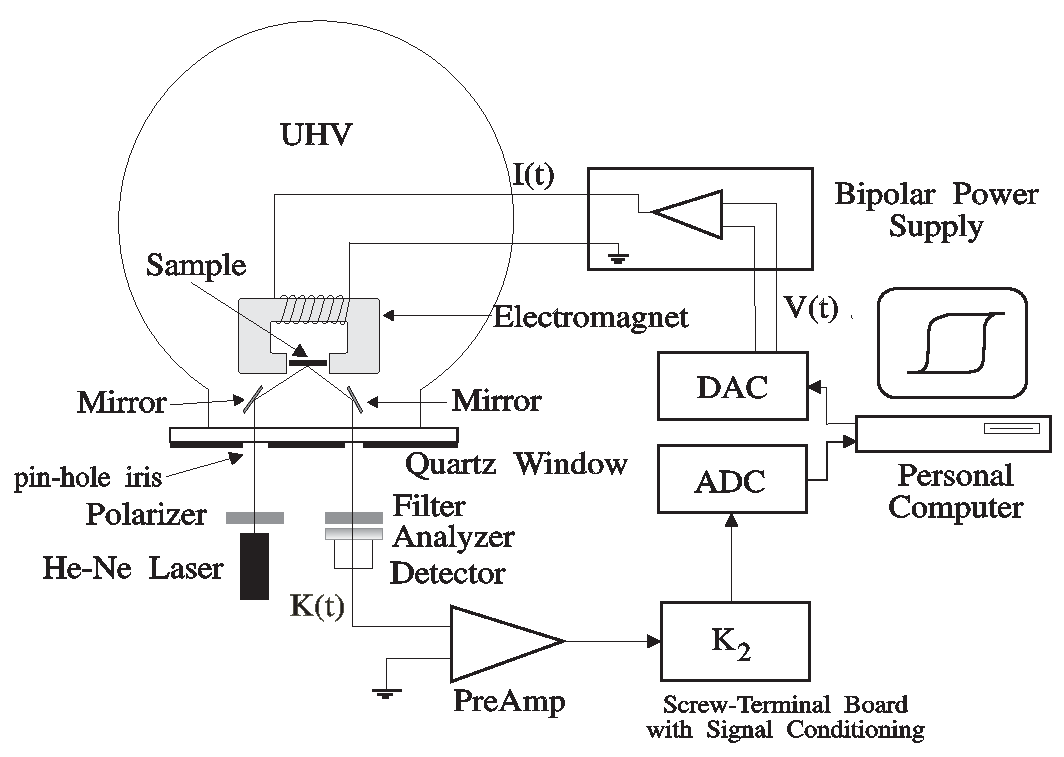
\includegraphics[width=.6\textwidth]{smokeblk}
    \caption{电路图}
    \label{fig:circuit-diagram}
\end{figure}

注意 \verb|figure| 环境是一个浮动体环境,图片的最终位置可能会跑动。\verb|[!h]| 中的 \verb|h| 是 here 的意思, \verb|!| 表示忽略一些浮动体的严格规则。另外里面还可以加上 \verb|btp| 选项,它们分别是 bottom, top, page 的意思。只要这几个参数在花括号里面,作用是不分先后顺序的。page 在这里表示浮动页。

\verb|\label{fig:circuit-diagram}| 是一个标签,供交叉引用使用的。例如引用图片 \verb|\cref{fig:circuit-diagram}| 的实际效果是\cref{fig:circuit-diagram}。图片是自动编号的,比起手动编号,它更加高效。\verb|\cref{label}| 由 \verb|cleveref| 宏包提供,比普通的 \verb|\ref{label}| 更加自动化。 \verb|label| 要确保唯一,命名方式推荐用图片的命名方式。

图片并排的需求解决方式多种多样,下面用 \verb|minipage| 环境来展示一个简单的例子。注意,以下例子用到了 \verb|subcaption| 命令,需要加载 subcaption 宏包。

\begin{figure}
    \centering
    \begin{minipage}[c]{0.3\textwidth}
        \centering
        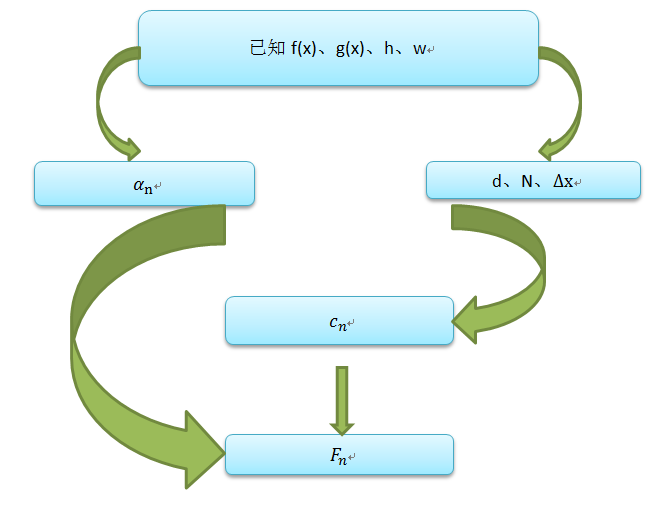
\includegraphics[width=0.95\textwidth]{f1}
        \subcaption{流程图}
        \label{fig:sample-figure-a}
    \end{minipage}
    \begin{minipage}[c]{0.3\textwidth}
        \centering
        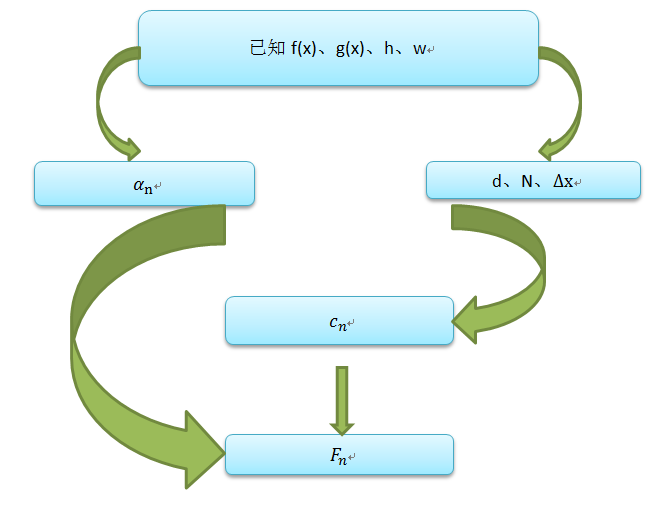
\includegraphics[width=0.95\textwidth]{f1}
        \subcaption{流程图}
        \label{fig:sample-figure-b}
    \end{minipage}
    \begin{minipage}[c]{0.3\textwidth}
        \centering
        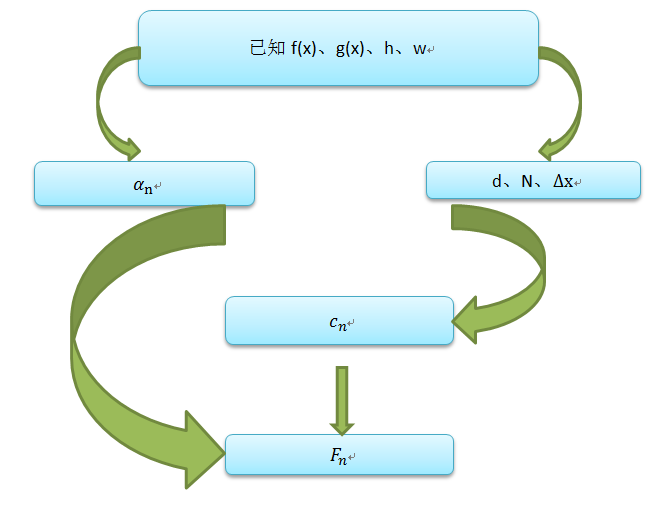
\includegraphics[width=0.95\textwidth]{f1}
        \subcaption{流程图}
        \label{fig:sample-figure-c}
    \end{minipage}
    \caption{多图并排示例}
    \label{fig:sample-figure}
\end{figure}
这相当于整体是一张大图片,大图片引用是\cref{fig:sample-figure},子图引用别分是\cref{fig:sample-figure-a}、\cref{fig:sample-figure-b}、\cref{fig:sample-figure-c}。

如果原本两张图片的高度不同,但是希望它们缩放后等高的排在同一行,参考这个例子:
\begin{figure}
    \centering
    \begin{minipage}[c]{0.48\textwidth}
        \centering
        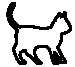
\includegraphics[height=0.2\textheight]{cat}
        \subcaption{一只猫}
    \end{minipage}
    \begin{minipage}[c]{0.48\textwidth}
        \centering
        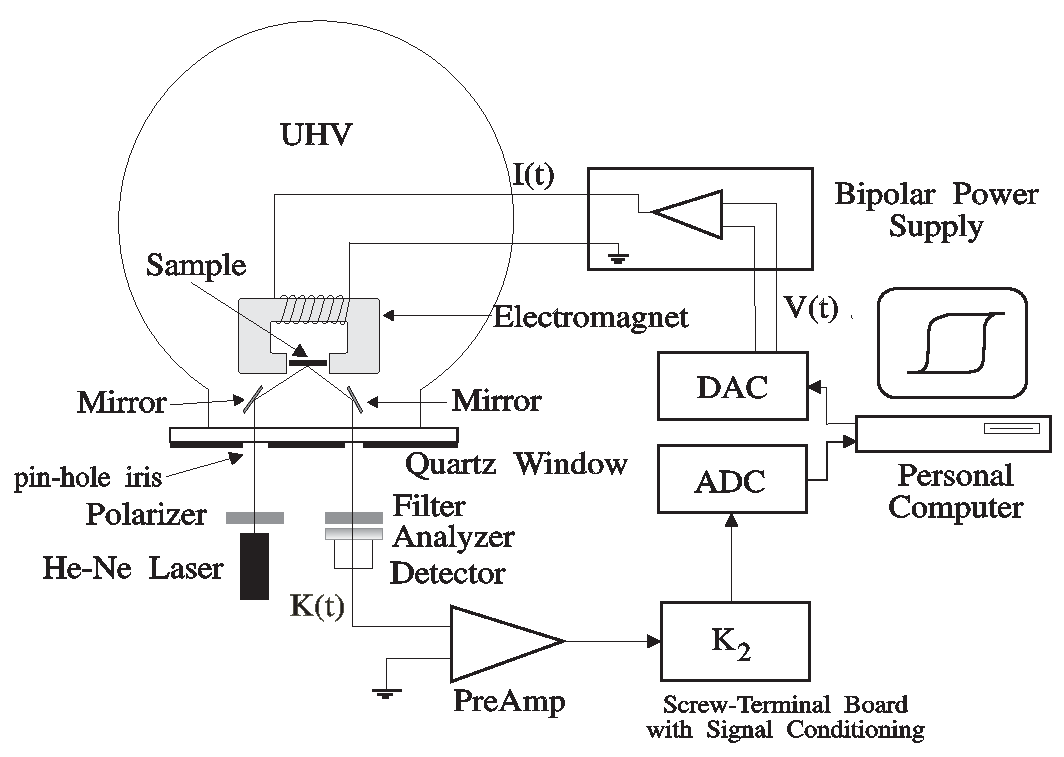
\includegraphics[height=0.2\textheight]{smokeblk}
        \subcaption{电路图}
    \end{minipage}
    \caption{多图并排示例}
\end{figure}

\section{绘制普通三线表格}
表格应具有三线表格式,因此常用 booktabs宏包,其标准格式如\cref{tab:001}~所示。
\begin{table}[!htbp]
    \caption{标准三线表格}\label{tab:001} \centering
    \begin{tabular}{ccccc}
        \toprule[1.5pt]
        $D$(in) & $P_u$(lbs) & $u_u$(in) & $\beta$ & $G_f$(psi.in) \\
        \midrule[1pt]
        5       & 269.8      & 0.000674  & 1.79    & 0.04089       \\
        10      & 421.0      & 0.001035  & 3.59    & 0.04089       \\
        20      & 640.2      & 0.001565  & 7.18    & 0.04089       \\
        \bottomrule[1.5pt]
    \end{tabular}
\end{table}

其绘制表格的代码及其说明如下。
\begin{tcode}
    \begin{table}[!htbp]
        \caption[标签名]{中文标题}
        \begin{tabular}{cc...c}
            \toprule[1.5pt]
            表头第1个格    & 表头第2个格    & ... & 表头第n个格                \\
            \midrule[1pt]
            表中数据(1,1) & 表中数据(1,2) & ... & 表中数据(1,n)             \\
            表中数据(2,1) & 表中数据(2,2) & ... & 表中数据(2,n)             \\
            ................................................... \\
            表中数据(m,1) & 表中数据(m,2) & ... & 表中数据(m,n)             \\
            \bottomrule[1.5pt]
        \end{tabular}
    \end{table}
\end{tcode}

\bigskip

table环境是一个将表格嵌入文本的浮动环境。tabular环境的必选参数由每列对应一个格式字符所组成:c表示居中,l表示左对齐,r表示右对齐,其总个数应与表的列数相同。此外,\verb|@{文本}|可以出现在任意两个上述的列格式之间,其中的文本将被插入每一行的同一位置。表格的各行以\verb|\\|分隔,同一行的各列则以\&分隔。 \verb|\toprule| 、\verb|\midrule| 和 \verb|\bottomrule| 三个命令是由booktabs宏包提供的,其中 \verb|\toprule| 和 \verb|\bottomrule| 分别用来绘制表格的第一条(表格最顶部)和第三条(表格最底部)水平线, \verb|\midrule| 用来绘制第二条(表头之下)水平线,且第一条和第三条水平线的线宽为 1.5pt ,第二条水平线的线宽为 1pt 。引用方法与图片的相同。

\section{公式}

数学建模必然涉及不少数学公式的使用。下面简单介绍一个可能用得上的数学环境。

首先是行内公式,例如 $ \theta $ 是角度。行内公式使用 \verb|$  $| 包裹。

行间公式不需要编号的可以使用 \verb|\[  \]| 包裹,例如
\[
    E=mc^2
\]
其中 $ E $ 是能量,$ m $ 是质量,$ c $ 是光速。

如果希望某个公式带编号,并且在后文中引用可以参考下面的写法:
\begin{equation}
    E=mc^2
    \label{eq:energy}
\end{equation}
式\cref{eq:energy}是质能方程。

多行公式有时候希望能够在特定的位置对齐,以下是其中一种处理方法。
\begin{align}
    P & = UI   \\
      & = I^2R
\end{align}
\verb|&| 是对齐的位置, \verb|&| 可以有多个,但是每行的个数要相同。

矩阵的输入也不难。
\[
    \mathbf{X} = \left(
    \begin{array}{cccc}
            x_{11} & x_{12} & \ldots & x_{1n} \\
            x_{21} & x_{22} & \ldots & x_{2n} \\
            \vdots & \vdots & \ddots & \vdots \\
            x_{n1} & x_{n2} & \ldots & x_{nn} \\
        \end{array} \right)
\]

分段函数这些可以用 \verb|case| 环境,但是它要放在数学环境里面。
\[
    f(x) =
    \begin{cases}
        0 & x \text{为无理数} , \\
        1 & x \text{为有理数} .
    \end{cases}
\]
在数学环境里面,字体用的是数学字体,一般与正文字体不同。假如要公式里面有个别文字,则需要把这部分放在 \verb|text| 环境里面,即 \verb|\text{文本环境}| 。

公式中个别需要加粗的字母可以用 \verb|$\bm{math symbol}$| 。如 $ \alpha a\bm{\alpha a} $ 。

以上仅简单介绍了基础的使用,对于更复杂的需求,可以阅读相关的宏包手册,如 \href{http://texdoc.net/texmf-dist/doc/latex/amsmath/amsldoc.pdf}{amsmath}。

希腊字母这些如果不熟悉,可以去查找符号文件 \href{http://mirrors.ctan.org/info/symbols/comprehensive/symbols-a4.pdf}{symbols-a4.pdf} ,也可以去 \href{http://detexify.kirelabs.org/classify.html}{detexify} 网站手写识别。另外还有数学公式识别软件 \href{https://mathpix.com/}{mathpix} 。

下面简单介绍一下定理、证明等环境的使用。
\begin{definition}
    定义环境
    \label{def:nosense}
\end{definition}
\cref{def:nosense}除了告诉你怎么使用这个环境以外,没有什么其它的意义。

除了 definition 环境,还可以使用 theorem 、lemma、corollary、assumption、conjecture、axiom、principle、problem、example、proof、solution 这些环境,根据论文的实际需求合理使用。

\begin{theorem}
    这是一个定理。
    \label{thm:example}
\end{theorem}
由\cref{thm:example}我们知道了定理环境的使用。

\begin{lemma}
    这是一个引理。
    \label{lem:example}
\end{lemma}
由\cref{lem:example}我们知道了引理环境的使用。

\begin{corollary}
    这是一个推论。
    \label{cor:example}
\end{corollary}
由\cref{cor:example}我们知道了推论环境的使用。

\begin{assumption}
    这是一个假设。
    \label{asu:example}
\end{assumption}
由\cref{asu:example}我们知道了假设环境的使用。

\begin{conjecture}
    这是一个猜想。
    \label{con:example}
\end{conjecture}
由\cref{con:example}我们知道了猜想环境的使用。

\begin{axiom}
    这是一个公理。
    \label{axi:example}
\end{axiom}
由\cref{axi:example}我们知道了公理环境的使用。

\begin{principle}
    这是一个定律。
    \label{pri:example}
\end{principle}
由\cref{pri:example}我们知道了定律环境的使用。

\begin{problem}
这是一个问题。
\label{pro:example}
\end{problem}
由\cref{pro:example}我们知道了问题环境的使用。

\begin{example}
    这是一个例子。
    \label{exa:example}
\end{example}
由\cref{exa:example}我们知道了例子环境的使用。

\begin{proof}
    这是一个证明。
    \label{prf:example}
\end{proof}
由\cref{prf:example}我们知道了证明环境的使用。

\begin{solution}
    这是一个解。
    \label{sol:example}
\end{solution}
由\cref{sol:example}我们知道了解环境的使用。



\section{其它小功能}
\subsection{脚注}

利用 \verb|\footnote{具体内容}| 可以生成脚注\footnote{脚注可以补充说明一些东西}。

\subsection{无序列表与有序列表}

无序列表是这样的:
\begin{itemize}
    \item one
    \item two
    \item ...
\end{itemize}

有序列表是这样子的:
\begin{enumerate}
    \item one
    \item two
    \item ...
\end{enumerate}

\subsection{字体加粗与斜体}

如果想强调部分内容,可以使用加粗的手段来实现。加粗字体可以用 \verb|\textbf{加粗}| 来实现。例如: \textbf{这是加粗的字体。 This is bold fonts} 。

中文字体没有斜体设计,但是英文字体有。\textit{斜体 Italics}。

\section{参考文献与引用}

参考文献对于一篇正式的论文来说是必不可少的,在建模中重要的参考文献当然应该列出。\LaTeX{}在这方面的功能也是十分强大的,下面进介绍一个比较简单的参考文献制作方法。有兴趣的可以学习 \verb|bibtex| 或 \verb|biblatex| 的使用。

\LaTeX{}的入门书籍可以看《\LaTeX{}入门》\cite{liuhaiyang2013latex}。这是一个简单的引用,用 \verb|\cite{bibkey}| 来完成。要引用成功,当然要维护好 bibitem 了。下面是个简单的例子。



%参考文献
\begin{thebibliography}{9}%宽度9
    \bibitem[1]{liuhaiyang2013latex}
    刘海洋.
    \newblock \LaTeX {}入门\allowbreak[J].
    \newblock 电子工业出版社, 北京, 2013.
    \bibitem[2]{mathematical-modeling}
    全国大学生数学建模竞赛论文格式规范 (2023 年 修改).
    \bibitem{3} \url{https://www.latexstudio.net}
\end{thebibliography}

\newpage
%附录
\begin{appendices}

    \section{模板所用的宏包}
    \begin{table}[htbp]
        \centering
        \caption{宏包罗列}
        \begin{tabular}{ccccc}
            \toprule
            \multicolumn{5}{c}{模板中已经加载的宏包}                                                           \\
            \midrule
            amsbsy         & amsfonts        & {amsgen}        & {amsmath}        & {amsopn}         \\
            amssymb        & amstext         & {appendix}      & {array}          & {atbegshi}       \\
            atveryend      & auxhook         & {bigdelim}      & {bigintcalc}     & {bigstrut}       \\
            bitset         & bm              & {booktabs}      & {calc}           & {caption}        \\
            caption3       & CJKfntef        & {cprotect}      & {ctex}           & {ctexhook}       \\
            ctexpatch      & enumitem        & {etexcmds}      & {etoolbox}       & {everysel}       \\
            expl3          & fix-cm          & {fontenc}       & {fontspec}       & {fontspec-xetex} \\
            geometry       & gettitlestring  & {graphics}      & {graphicx}       & {hobsub}         \\
            hobsub-generic & hobsub-hyperref & {hopatch}       & {hxetex}         & {hycolor}        \\
            hyperref       & ifluatex        & {ifpdf}         & {ifthen}         & {ifvtex}         \\
            ifxetex        & indentfirst     & {infwarerr}     & {intcalc}        & {keyval}         \\
            kvdefinekeys   & kvoptions       & {kvsetkeys}     & {l3keys2e}       & {letltxmacro}    \\
            listings       & longtable       & {lstmisc}       & {ltcaption}      & {ltxcmds}        \\
            multirow       & nameref         & {pdfescape}     & {pdftexcmds}     & {refcount}       \\
            rerunfilecheck & stringenc       & {suffix}        & {titletoc}       & {tocloft}        \\
            trig           & ulem            & {uniquecounter} & {url}            & {xcolor}         \\
            xcolor-patch   & xeCJK           & {xeCJKfntef}    & {xeCJK-listings} & {xparse}         \\
            xtemplate      & zhnumber        &                 &                  &                  \\
            \bottomrule
        \end{tabular}%
        \label{tab:addlabel}%
    \end{table}%

    以上宏包都已经加载过了,不要重复加载它们。

    \section{排队算法--matlab 源程序}

    \begin{lstlisting}[language=matlab]
kk=2;[mdd,ndd]=size(dd);
while ~isempty(V)
[tmpd,j]=min(W(i,V));tmpj=V(j);
for k=2:ndd
[tmp1,jj]=min(dd(1,k)+W(dd(2,k),V));
tmp2=V(jj);tt(k-1,:)=[tmp1,tmp2,jj];
end
tmp=[tmpd,tmpj,j;tt];[tmp3,tmp4]=min(tmp(:,1));
if tmp3==tmpd, ss(1:2,kk)=[i;tmp(tmp4,2)];
else,tmp5=find(ss(:,tmp4)~=0);tmp6=length(tmp5);
if dd(2,tmp4)==ss(tmp6,tmp4)
ss(1:tmp6+1,kk)=[ss(tmp5,tmp4);tmp(tmp4,2)];
else, ss(1:3,kk)=[i;dd(2,tmp4);tmp(tmp4,2)];
end;end
dd=[dd,[tmp3;tmp(tmp4,2)]];V(tmp(tmp4,3))=[];
[mdd,ndd]=size(dd);kk=kk+1;
end; S=ss; D=dd(1,:);
 \end{lstlisting}

    \section{规划解决程序--lingo源代码}

    \begin{lstlisting}[language=c]
kk=2;
[mdd,ndd]=size(dd);
while ~isempty(V)
    [tmpd,j]=min(W(i,V));tmpj=V(j);
for k=2:ndd
    [tmp1,jj]=min(dd(1,k)+W(dd(2,k),V));
    tmp2=V(jj);tt(k-1,:)=[tmp1,tmp2,jj];
end
    tmp=[tmpd,tmpj,j;tt];[tmp3,tmp4]=min(tmp(:,1));
if tmp3==tmpd, ss(1:2,kk)=[i;tmp(tmp4,2)];
else,tmp5=find(ss(:,tmp4)~=0);tmp6=length(tmp5);
if dd(2,tmp4)==ss(tmp6,tmp4)
    ss(1:tmp6+1,kk)=[ss(tmp5,tmp4);tmp(tmp4,2)];
else, ss(1:3,kk)=[i;dd(2,tmp4);tmp(tmp4,2)];
end;
end
    dd=[dd,[tmp3;tmp(tmp4,2)]];V(tmp(tmp4,3))=[];
    [mdd,ndd]=size(dd);
    kk=kk+1;
end;
S=ss;
D=dd(1,:);
 \end{lstlisting}
\end{appendices}


\end{document}\end{document}